
In this exercise we implement a multiclass classification problem with a Decision Tree.
We start from the binary case and extend it to the multiclass problem.\\
The parameter to be optimized in this problem can be the depth of the tree.\\
Also in this case we divide the dataset into two sets, the learning set and the validation set and using the validation set we calculate the error as the number of points classified incorrectly. Here again we repeat the product k times, with k equal to 30.\\

\begin{figure}[h]
\centering
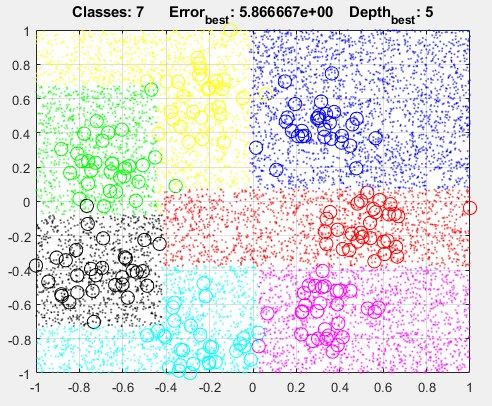
\includegraphics[width=0.5\textwidth]{i3.png}
\caption{Regression Function}
\label{fig:regression function}
\end{figure}
\begin{figure}[h]
Finally, we took a dataset with 3 features, in order to be plottable in 3D, and 3 classes. 
As before we divided dataset in training set and validation set, we used $ 70\%$ of data in training and the remaining for validation. Then we ran a loop on k and on depth to optimize the depth parameter.\\ \\ \\ \\


	\centering
	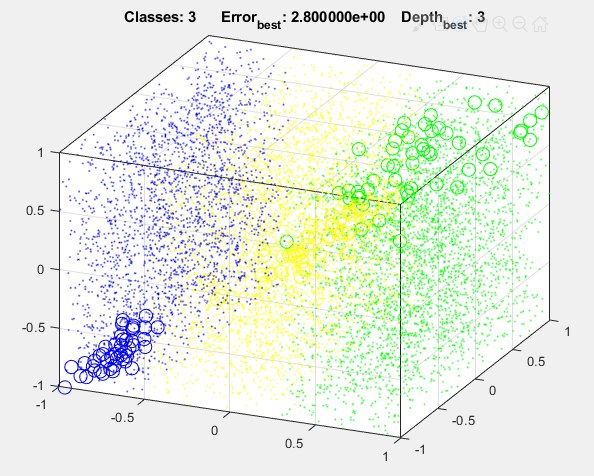
\includegraphics[width=1\textwidth]{i4.png}
	\caption{Regression Function}
	\label{fig:regression function}
\end{figure}
